\documentclass[
11pt, % The default document font size, options: 10pt, 11pt, 12pt
%codirector, % Uncomment to add a codirector to the title page
]{charter} 


% El títulos de la memoria, se usa en la carátula y se puede usar el cualquier lugar del documento con el comando \ttitle
\titulo{Proyección del índice de vegetación de diferencia normalizada satelital de cebada en crecimiento con series temporales e inteligencia artificial} 

% Nombre del posgrado, se usa en la carátula y se puede usar el cualquier lugar del documento con el comando \degreename
%\posgrado{Carrera de Especialización en Sistemas Embebidos} 
%\posgrado{Carrera de Especialización en Internet de las Cosas} 
\posgrado{Carrera de Especialización en Inteligencia Artificial}
%\posgrado{Maestría en Sistemas Embebidos} 
%\posgrado{Maestría en Internet de las cosas}

% Tu nombre, se puede usar el cualquier lugar del documento con el comando \authorname
% IMPORTANTE: no omitir titulaciones ni tildación en los nombres, también se recomienda escribir los nombres completos (tal cual los tienen en su documento)
\autor{Dr. Ing. Agr. Adrián Lapaz Olveira}

% El nombre del director y co-director, se puede usar el cualquier lugar del documento con el comando \supname y \cosupname y \pertesupname y \pertecosupname
\director{Esp. Lic. Maria Carina Roldán}
\pertenenciaDirector{FIUBA} 
\codirector{Esp. Ing. Ariadna Garmendia} % para que aparezca en la portada se debe descomentar la opción codirector en los parámetros de documentclass
\pertenenciaCoDirector{FIUBA}

% Nombre del cliente, quien va a aprobar los resultados del proyecto, se puede usar con el comando \clientename y \empclientename
\cliente{PhD. MSc. Ing. Agr. Andrés Berger}
\empresaCliente{INIA}
 
\fechaINICIO{4 de marzo de 2025}		%Fecha de inicio de la cursada de GdP \fechaInicioName
\fechaFINALPlan{22 de abril de 2025} 	%Fecha de final de cursada de GdP
\fechaFINALTrabajo{agosto de 2025}	%Fecha de defensa pública del trabajo final


\begin{document}

\maketitle
\thispagestyle{empty}
\pagebreak


\thispagestyle{empty}
{\setlength{\parskip}{0pt}
\tableofcontents{}
}
\pagebreak


\section*{Registros de cambios}
\label{sec:registro}


\begin{table}[ht]
\label{tab:registro}
\centering
\begin{tabularx}{\linewidth}{@{}|c|X|c|@{}}
\hline
\rowcolor[HTML]{C0C0C0} 
Revisión & \multicolumn{1}{c|}{\cellcolor[HTML]{C0C0C0}Detalles de los cambios realizados} & Fecha      \\ \hline
0      & Creación del documento                                 &\fechaInicioName \\ \hline
1      & Se completa hasta el punto 5 inclusive                & {20} de {marzo} de 2025 \\ \hline
2      & Se completa hasta el punto 5 inclusive               & {28} de {marzo} de 2025 \\
\hline
%		  Se puede agregar algo más \newline
%		  En distintas líneas \newline
%		  Así                                                    & {día} de {mes} de 202X \\ \hline
3      & Se completa hasta el punto 12 inclusive                & {1} de {abril} de 2025 \\ \hline
%4      & Se completa el plan	                                 & {día} de {mes} de 202X \\ \hline
4      & Se completa hasta el punto 15 inclusive                & {11} de {abril} de 2025 \\ \hline
%5      & Se completa el plan	                                 & {20} de {abril} de 2025 \\ \hline

% Si hay más correcciones pasada la versión 4 también se deben especificar acá

\end{tabularx}
\end{table}

\pagebreak



\section*{Acta de constitución del proyecto}
\label{sec:acta}

\begin{flushright}
Buenos Aires, \fechaInicioName
\end{flushright}

\vspace{2cm}

Por medio de la presente se acuerda con el \authorname\hspace{1px} que su Trabajo Final de la \degreename\hspace{1px} se titulará ``\ttitle'' y consistirá en la predicción temprana del índice de vegetación de diferencia normalizada máximo de los cultivos de cebada, a través del uso series temporales de datos Sentinel-2 y modelos de inteligencia artificial para las campañas 2023-2025. El trabajo tendrá un presupuesto preliminar estimado de 650 horas y un costo estimado de UYU 2.363.366 (pesos uruguayos), financiado conjuntamente por INIA (UY), AmBev (UY) y ANII (UY)* en el marco de un proyecto de articulación. La fecha de inicio el \fechaInicioName\hspace{1px} y fecha de presentación pública en \fechaFinalName.

Se adjunta a esta acta la planificación inicial.

\vfill

% Esta parte se construye sola con la información que hayan cargado en el preámbulo del documento y no debe modificarla
\begin{table}[ht]
\centering
\begin{tabular}{ccc}
\begin{tabular}[c]{@{}c@{}}Dr. Ing. Ariel Lutenberg \\ Director posgrado FIUBA\end{tabular} & \hspace{2cm} & \begin{tabular}[c]{@{}c@{}}\clientename \\ \empclientename \end{tabular} \vspace{2.5cm} \\ 
\multicolumn{3}{c}{\begin{tabular}[c]{@{}c@{}} \supname \\ Director del Trabajo Final\end{tabular}} \vspace{2.5cm} \\
\end{tabular}
\end{table}

\pagebreak



\section{1. Descripción técnica-conceptual del proyecto a realizar}
\label{sec:descripcion}

\subsection{Antecedentes}
\label{sec:descripcion}
La producción de cebada (\emph{Hordeum vulgare L.}) con destino industrial tiene como objetivo maximizar el rendimiento con una concentración de proteína en grano del 9{,}5 al 12{,}5 \% (MacLeod s.f.; Hu et al. 2021; Reussi Calvo et al. 2022). Para alcanzar este objetivo, es esencial realizar un diagnóstico temprano y preciso de los nutrientes para garantizar un crecimiento sin restricciones a lo largo de todo el ciclo del cultivo, sin sub o sobrefertilización (Baethgen y Christianson 1995; Araújo et al. 2022). No obstante, la principal dificultad para alcanzar este objetivo es la falta de precisión en el diagnóstico actual, ya que, al estar basado en determinaciones a la siembra, emergencia y/o estadíos iniciales del cultivo, este no contempla cómo los factores climáticos afectan el crecimiento de las plantas, y en consecuencia, cambian el rendimiento potencial y la demanda nutricional futura (Pettersson y Eckersten 2007; Cammarano et al. 2024; Halstead et al. 2022). Por lo tanto, el diagnóstico nutricional actual de cebada demanda herramientas complementarias que permitan proyectar el crecimiento potencial del cultivo.
 
Una de las herramientas calibradas para proyectar el crecimiento de los cultivos es la función $\beta$ (Yin et al. 2003; Beck et al. 2006). Al modelar la acumulación de biomasa según los días desde la siembra (DDS), sus parámetros son biológicamente interpretables, lo que facilita su adopción en modelos de simulación de cultivos (Reussi Calvo et al. 2022). Sin embargo, su parametrización demanda determinaciones de biomasa durante el desarrollo fenológico, que representa una desventaja para su adopción por parte de los productores y asesores (Bending et al. 2014). La determinación de la biomasa consiste en colectar plantas a campo para luego secarlas en laboratorio; por consiguiente, su procedimiento demanda mucho tiempo, es costoso y tiene limitada representatividad a escala de lote (Berger et al. 2013). Por lo tanto, el uso de indicadores relacionados con la biomasa permitiría proyectar el crecimiento del cultivo a través del ajuste de una función $\beta$ y, en consecuencia, predecir la demanda nutricional futura.

La disponibilidad de tecnologías emergentes de teledetección satelital permite estimar in situ diversos parámetros biofísicos y químicos de los cultivos de forma rápida, sin costo y a escala de lote (Campbell, 2022; Lapaz Olveira, 2023; Morris et al., 2018). En esta línea, el uso de datos abiertos de la misión satelital de Sentinel-2 observa la energía electromagnética terrestre a una alta resolución temporal ($\mathbb{<}7$ días), espectral (+3 bandas) y espacial ($10$ o $20$ m de píxel cuadrado), lo cual permitiría proyectar de forma precisa el crecimiento del cultivo (ESA, 2025). Específicamente, estas observaciones se utilizan para calcular el Índice de Vegetación de Diferencia Normalizada (NDVI), que es un indicador directo del vigor de las plantas y, en efecto, un estimador de los parámetros biofísicos de los cultivos (Reussi Calvo et al. 2022; Bending et al. 2014). Por lo tanto, si el NDVI presenta una dinámica similar a la acumulación de la biomasa, su proyección con la función $\beta$ aumentaría la precisión del diagnóstico nutricional al estimar el crecimiento potencial del cultivo.

Para llevar a cabo este ajuste de la función $\beta$ y estimar sus parámetros a partir de observaciones iniciales de NDVI, es especialmente adecuado utilizar la inferencia bayesiana (Yin et al. 2003; Paruelo et al. 2024). Bajo este enfoque, se parte de un conocimiento inicial acerca de los parámetros (representado por una distribución previa, \emph{priors}) y se actualiza dicha información conforme se obtienen más mediciones de NDVI a lo largo del ciclo de cultivo (Guszcza 2008; Bürkner 2018; Martin 2024). De esta manera, la distribución posterior de los parámetros de la función $\beta$ (como los descritos originalmente por Yin et al., 2003) reduce su dispersión, lo que aumenta la precisión en la proyección del NDVI. Este proceso no solo aprovecha los datos iniciales para predecir el crecimiento potencial, sino que también permite incorporar ajustes a medida que surgen nuevas observaciones de NDVI (Guszcza 2008; Bürkner 2018; Martin 2024). Por lo tanto, la precisión del enfoque bayesiano para predecir el NDVI potencial del cultivo aumenta con el ciclo fenológico, y en efecto, también la precisión del diagnóstico nutricional.

En la actualidad, la inteligencia artificial es utilizada exitosamente para monitorear diversos parámetros biofísicos y químicos en cultivos y pasturas (Yoosefzadeh-Najafabadi et al. 2021; Farbo et al., 2025). Estudios previos han utilizado eficazmente datos históricos de NDVI, temperaturas y precipitación para predecir valores futuros del índice (Cavalli et al., 2023). En esta línea de investigación, un estudio reportó que las redes neuronales artificiales (ANN) predicen con precisión el NDVI futuro de maíz (\emph{Zea mays L.}) en el corto plazo (5–15 días) (Farbo et al., 2025). En este estudio, las ANN fueron entrenadas con el NDVI, índice de diferencia de agua normalizado (NDWI), precipitaciones acumuladas (GPM) y grados días acumulados (AGDD). Cabe mencionar que, además de estas variables agroclimáticas, existen otras que determinan el crecimiento de la cebada, como el coeficiente fototermal (Q) y fotoperíodo (P) (Hu et al., 2003; Reussi Calvo et al., 2022). También son determinantes las variables de manejo como el cultivar, fecha de siembra y dosis de nitrógeno (N) (Baethgen et al., 1995; Araújo et al., 2022). Por otro lado, en pasturas de campo natural se ha demostrado que el NDVI puede predecirse en el largo plazo (1–3 meses) (Paruelo et al., 2024). Esto se ha logrado a través del desarrollo de modelos híbridos, que proyectan la producción primaria neta con modelos paramétricos sigmoideos, similares a la función $\beta$ (Yin et al. 2003), y usan algoritmos de ANN para estimar los errores de esta proyección (Martin 2024). Por lo tanto, los modelos híbridos que estimen mediante ANN los errores de la proyección bayesiana de la función $\beta$ incrementarán la exactitud predictiva del NDVI potencial y optimizarán el diagnóstico nutricional del cultivo.

A pesar de que se ha demostrado que el NDVI es un fiel indicador del crecimiento de las plantas, su proyección durante el ciclo del cultivo aún no ha sido investigada en profundidad, lo cual limita la precisión del diagnóstico temprano. Esta falta de investigación representa una oportunidad para mejorar la capacidad de predecir el desarrollo de los cultivos y optimizar su manejo. Por lo tanto, este trabajo tiene como objetivo i) predecir el NDVI potencial del cultivo a partir de observaciones realizadas desde la siembra hasta los 45, 60 y 75 DDS, y ii) evaluar si las variables agroclimáticas y de manejo contribuyen a mejorar la precisión en la estimación del índice (Bayes vs modelo híbrido).

\subsection{Metodología}
\label{sec:descripcion}
La figura~\ref{fig:Flujo_de_Trabajo} representa el flujo de trabajo desarrollado para predecir el NDVI potencial en lotes comerciales de cebada maltera durante las campañas 2023 y 2024. El procedimiento se inicia con la recopilación de información agronómica y espacial, representada mediante polígonos georreferenciados (formato JSON), que incluyen la fecha de siembra, el cultivar seleccionado y la dosis de N aplicada (kg ha$^{-1}$). Esta información sirve como base para extraer, de forma concurrente, datos meteorológicos y satelitales. 

El conjunto de datos se dividirá de acuerdo con su objetivo analítico: los registros correspondientes a la campaña 2023 se destinarán a la calibración del modelo, mientras que los de la campaña 2024 se utilizarán para su validación. A su vez, cada conjunto se truncará en tres momentos clave del ciclo del cultivo: 45, 60 y 75 DDS, incorporando también variables previas al evento de siembra (hasta -5 DDS). De este modo, se simularán diferentes escenarios de disponibilidad temporal de información para evaluar la capacidad predictiva del modelo.

La primera etapa del modelado consistirá en el ajuste de una función de crecimiento $\beta$ a las observaciones de NDVI en función de DDS. Esta función permite capturar la dinámica estacional del desarrollo del cultivo mediante parámetros con interpretación biológica como $w_{max}$ (ver sección 1.2.3.). A partir de este ajuste se obtendrán las predicciones iniciales del NDVI potencial para cada horizonte temporal.

A continuación, se calcularán los residuales como la diferencia entre los valores observados y los estimados por el modelo sigmoideo. Estos residuales se utilizarán como variable respuesta para entrenar una ANN, alimentada con variables agroclimáticas y de manejo agrícola. La ANN se ajustará mediante validación cruzada, utilizando un 75 \% de los datos para entrenamiento y el 25 \% restante para validación, y se aplicarán técnicas de regularización para reducir el riesgo de sobreajuste.

Finalmente, se integrarán el modelo paramétrico y la ANN en un esquema de modelado híbrido. Esta estrategia busca aprovechar la capacidad explicativa de la curva de crecimiento, basada en los principios de la dinámica vegetal, junto con la flexibilidad de las ANN para capturar respuestas no lineales del cultivo frente a condiciones ambientales variables. El modelo híbrido será evaluado utilizando los datos de la campaña 2024 en los tres horizontes definidos, y su precisión se medirá a partir de la diferencia entre el NDVI potencial proyectado y el observado.


\begin{figure}[htpb]
\centering 
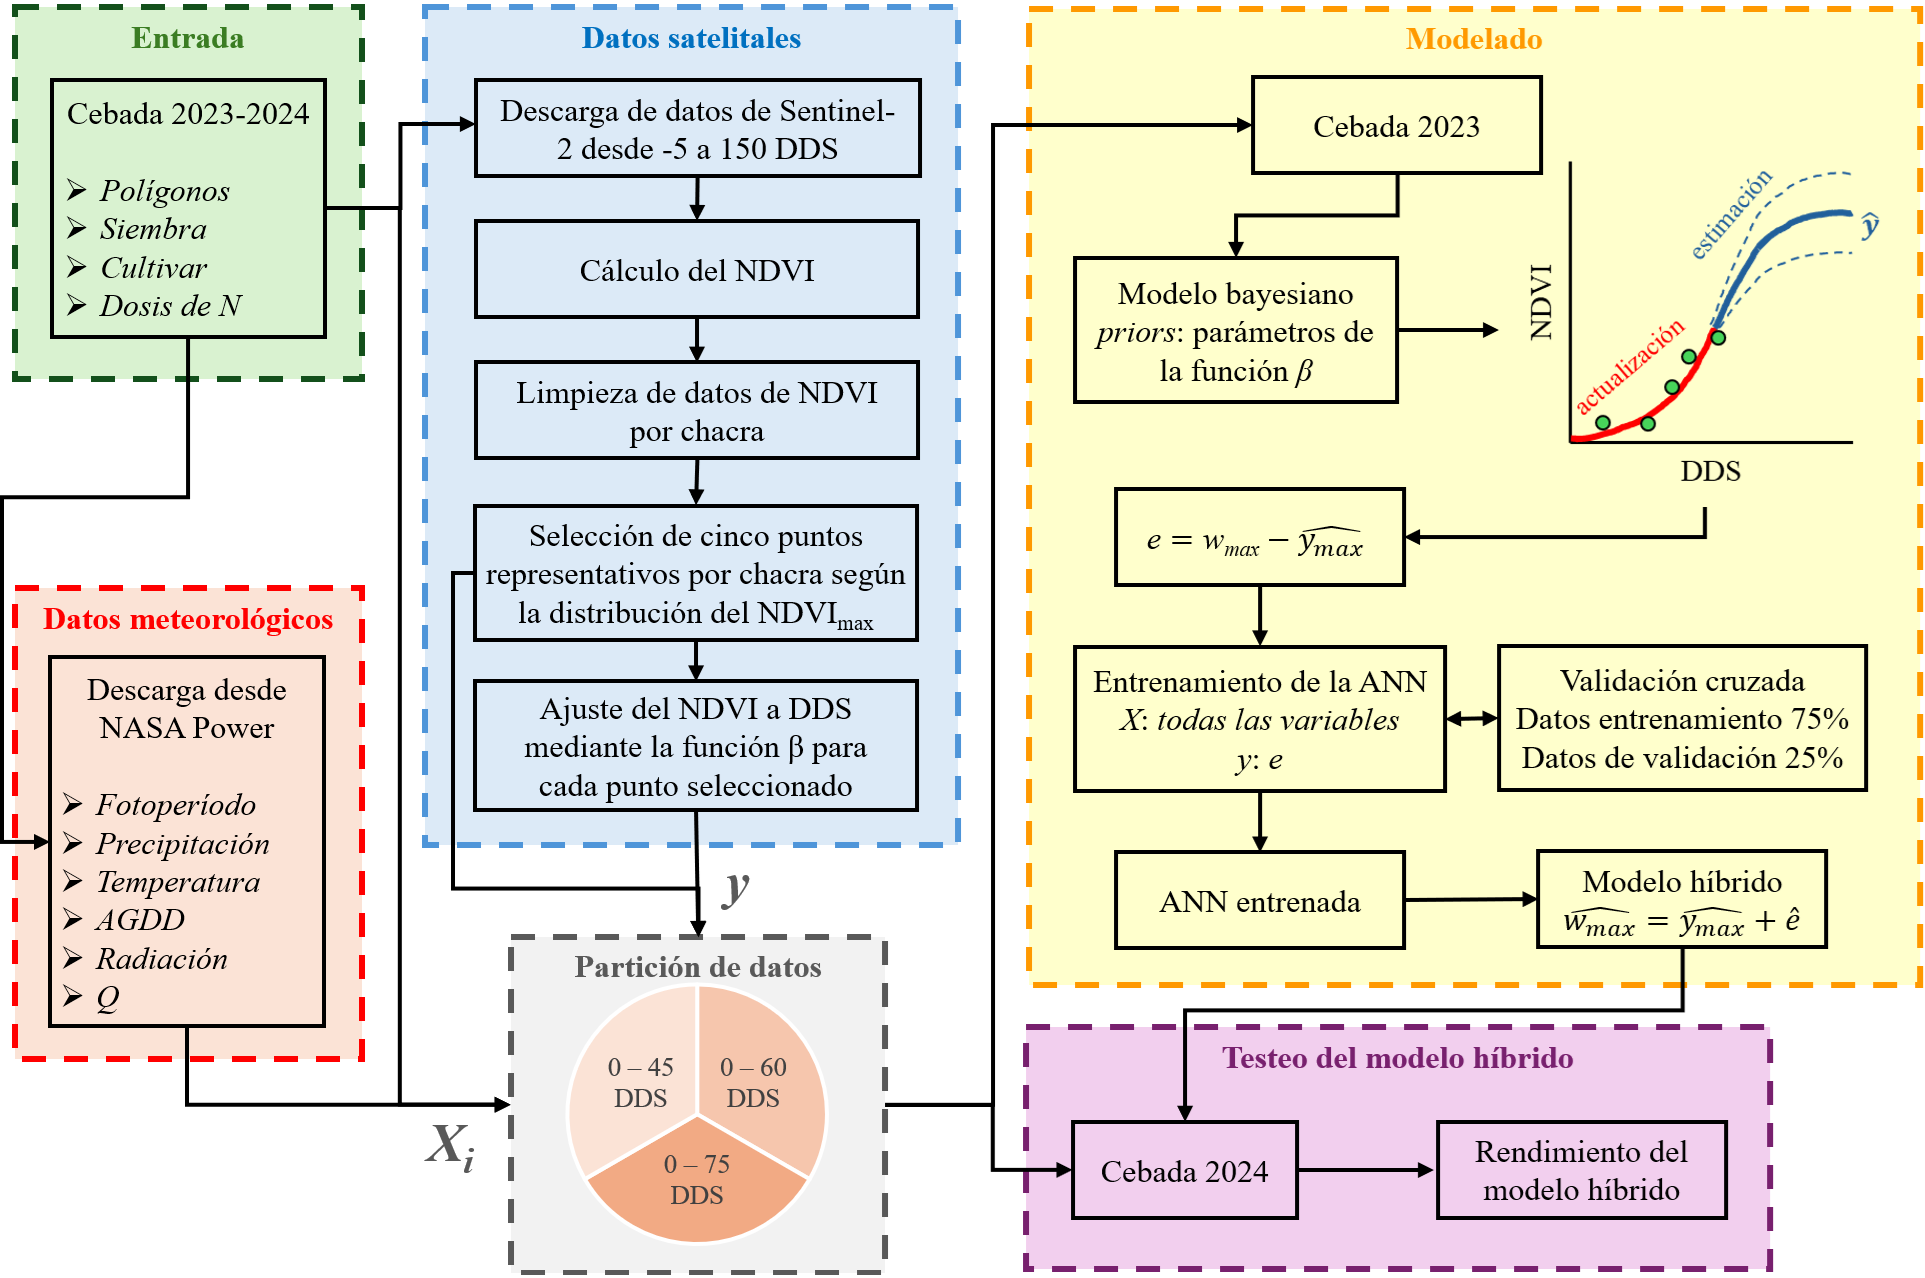
\includegraphics[width=.99\textwidth]{./Figuras/Flujo_de_Trabajo.png}
\caption{Diagrama del flujo de trabajo. N: nitrógeno; Q: coeficiente fototermal; DDS: días desde la siembra; NDVI: índice de vegetación de diferencia normalizada; NDVI$_{\max}$: valor máximo del NDVI; \emph{priors}: distribuciones a priori; $w_{\max}$: parámetro de la función $\beta$ que representa la máxima acumulación de biomasa; $\hat{y}_{\max}$: valor máximo estimado mediante proyección bayesiana; \emph{e}: error; ANN: red neuronal artificial.}

\label{fig:Flujo_de_Trabajo}
\end{figure}


\subsubsection{Datos agrometeorológicos}
\label{sec:descripcion}
Dado el amplio alcance geográfico y la necesidad de contar con datos bianuales, los datos agrometeorológicos serán obtenidos a través de la API RESTful de \textit{NASA POWER}, por medio del cliente \textit{PyNASApower} (en lenguaje Python, versión 3.13). El punto de consulta será el centroide de cada lote. Entre las variables recopiladas a diario se incluirán la precipitación (PP), temperatura (T), fotoperíodo (P) y radiación (R). A partir de estas variables, se calcularán para cada día ($i$-ésimo) hasta el último día disponible ($n$), la precipitación global acumulada (GPM), los grados día de crecimiento acumulados (AGDD) y el coeficiente fototermal (Q).

\begin{equation}
\label{eq:GPM}
\text{GPM} = \sum_{i=1}^{n} PP_{i}
\end{equation}

\begin{equation}
\label{eq:AGDD}
\text{AGDD} = \sum_{i=1}^{n} GDD_{i}
\end{equation}

\begin{equation}
\label{eq:Q}
Q_i = \frac{R_i}{T_i - T_{\text{base}}}
\end{equation}


\subsubsection{Datos satelitales}
\label{sec:descripcion}

Para procesar eficientemente los datos de reflectancia superficial corregidos geométrica y radiométricamente en una amplia área geográfica durante las campañas de cebada 2023–2024, se accederá al conjunto de datos \textit{Harmonized Sentinel-2 MSI Level-2A}, disponible a través del \textit{Earth Engine Data Catalog}, mediante la API de Python de \textit{Earth Engine} (versión 3.13 de Python). Este conjunto de datos ofrecerá una resolución espacial de 10 metros de pixel, una resolución radiométrica de 12 bits y una precisión posicional de aproximadamente 3 metros. Dentro de cada lote, se calculará el NDVI  como
la diferencia normalizada entre la reflectancia ($\rho$) en el infrarrojo cercano (833 nm, $\pm$ 106 nm, pixel 10 m) y en el rojo (665 nm, $\pm$ 31 nm, pixel 10 m) (ESA, 2025). 

\begin{equation}
\text{NDVI} = \frac{\rho_{\text{infrarrojo}} - \rho_{\text{rojo}}}{\rho_{\text{infrarrojo}} + \rho_{\text{rojo}}} \label{eq:ndvi_def}
\end{equation}

Una vez obtenida la serie temporal de NDVI para cada píxel, se calcularán los valores mínimos y máximos de NDVI correspondientes a cada píxel del lote durante el período de crecimiento del cultivo. Este procedimiento permitirá filtrar aquellos píxeles que no representen al cultivo de interés. Para ello, se eliminarán los píxeles cuyos valores máximos de NDVI no superen el umbral de 0,5, como ocurre en superficies de suelo desnudo, donde los valores suelen ser consistentemente bajos. También se descartarán aquellos píxeles cuyos valores mínimos no sean inferiores a 0,4, ya que en coberturas permanentes, como montes o vegetación densa, el NDVI tiende a mantenerse por encima de ese valor. Luego, se excluirán los registros que presenten una disminución superior al 10 \% respecto al valor registrado en la fecha anterior. Este tipo de caída abrupta podría estar relacionada con condiciones atmosféricas adversas, como nubosidad, o con eventos antrópicos puntuales, como el pastoreo o la recolección de plantas para heno. Una vez aplicados estos filtros, se obtendrá una serie de valores de NDVI depurados, adecuada para su posterior análisis estadístico.

\subsubsection{Función $\beta$}
\label{sec:descripcion}

Dado que el comportamiento del NDVI a lo largo del ciclo de crecimiento del cultivo presenta una dinámica similar a la de las plantas, se ajustará la función $\beta$ dado que modela con precisión la acumulación de biomasa en función de los DDS (Yin et al., 2003). A diferencia de otros modelos sigmoides, esta función incorpora parámetros biológicamente interpretables, como se muestra en la figura \ref{fig:Curva_Beta }. Además, su estructura matemática permite modelar de manera continua la evolución de la biomasa sin generar discontinuidades en la transición entre fases de crecimiento, lo que proporcionará estimaciones más realistas y ajustadas a la naturaleza determinante del crecimiento de estos cultivos. Por lo tanto, la parametrización de la dinámica del NDVI mediante la función $\beta$ ofrece una estrategia promisoria para la proyección temprana de la biomasa acumulada en cebada.

La significancia de estos parámetros radica en su capacidad para representar con alta fidelidad la trayectoria sigmoidal inherente al proceso de crecimiento. Concretamente, posibilitan la discriminación cuantitativa de la fase inicial de desarrollo, caracterizada por una tasa de incremento gradual; el período intermedio de expansión acelerada, donde la acumulación de biomasa exhibe su máxima velocidad; y la fase final de atenuación, marcada por una progresiva estabilización en los valores de la variable de crecimiento. 

La ecuación para calcular estos parámetros mediante mínimos cuadrados no lineales (nls) es la siguiente

\begin{equation}
\label{eq:betaGrowth}
w = w_b \;+\; \bigl(w_{\max} - w_b\bigr) 
        \left(1 + \frac{t_e - t}{t_e - t_m}\right)
        \left(\frac{t - t_b}{t_e - t_b}\right)^{\!\frac{t_m - t_b}{t_e - t_m}}
\end{equation}

sujeto a la condición \(t_b \;\leq\; t_m \;<\; t_e\).

\begin{figure}[htpb]
    \centering
    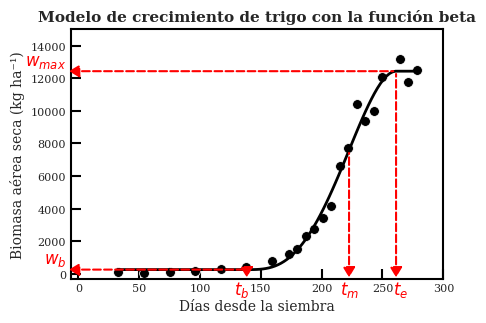
\includegraphics[width=.5\textwidth]{./Figuras/Curva_Beta.png}
    \caption{Dinámica temporal observada (puntos) y ajustada mediante la función de crecimiento beta (curva) de la biomasa aérea seca en trigo de invierno (datos de Gregory et al., 1978 citado por Yin et al., 2003). Los parámetros de la función beta son los siguientes, $w_b$: biomasa inicial; $w_{\max}$: biomasa máxima alcanzada; $t_b$: tiempo de inicio del crecimiento significativo; $t_m$: punto de inflexión (tasa de crecimiento máxima); $t_e$: tiempo en el que finaliza el crecimiento.}
    \label{fig:Curva_Beta }
\end{figure}

\subsubsection{NDVI potencial}
\label{sec:NDVI_potencial}

Dada la estrecha relación entre la dinámica del crecimiento del cultivo y la evolución del NDVI, se considerará al NDVI potencial como la variable más adecuada para realizar predicciones relevantes en el diagnóstico nutricional de la cebada. Este análisis se basará en series temporales de datos NDVI que abarcarán la totalidad del ciclo fenológico del cultivo durante las campañas 2023 y 2024.

Una vez obtenida la serie temporal de NDVI para cada píxel, se calculará el valor máximo de NDVI correspondiente. Esto permitirá generar un mapa de NDVI máximo con una resolución espacial de 10 metros. A partir de dicho mapa, se analizará la distribución de los valores con el objetivo de identificar las cinco ubicaciones más representativas dentro de cada lote. Estas corresponderán al valor mínimo, al valor máximo y a los percentiles 25, 50 y 75 de la distribución del NDVI máximo.

Este enfoque permitirá capturar de manera robusta la variabilidad y los contrastes espaciales del NDVI máximo a escala de lote. Posteriormente, sobre estos cinco puntos seleccionados en cada lote, se trabajará con la serie temporal de NDVI en función de los DDS, con el propósito de estimar, mediante mínimos cuadrados lineales, los parámetros de la función $\beta$. En este contexto, el parámetro $w_{\text{max}}$ se interpretará como el NDVI potencial de cada píxel seleccionado.


\subsubsection{Modelo bayesiano}
\label{sec:modelo_bayesiano}

Para estimar el NDVI potencial a partir de observaciones parciales de la serie temporal del cultivo, se implementará un modelo jerárquico bayesiano no lineal, estructurado en tres niveles: observacional, de proceso y de parámetros. Este modelo se basa en la función de crecimiento tipo $\beta$, utilizada previamente en ecología y ciencia actuarial para representar trayectorias sigmoideas (Clark, 2003; Guszcza, 2008).

\paragraph{Nivel observacional.} El valor de NDVI observado en el tiempo \( t \) para el píxel \( i \) se modela como una variable aleatoria con error gaussiano:

\begin{equation}
\text{NDVI}_{i,t} \sim \mathcal{N}(\hat{w}_{i,t}, \sigma^2)
\end{equation}

donde \( \hat{w}_{i,t} \) representa el valor estimado por la función de crecimiento beta.

\paragraph{Nivel de proceso.} La evolución temporal de \( \hat{w}_{i,t} \) se describe mediante la función $\beta$:

\begin{equation}
\hat{w}_{i,t} = w_b + (w_{\max,i} - w_b) 
\left( 1 + \frac{t_e - t}{t_e - t_m} \right)
\left( \frac{t - t_b}{t_e - t_b} \right)^{\frac{t_m - t_b}{t_e - t_m}}
\end{equation}

\noindent
sujeta a la condición asintótica que refleja la estabilización del dosel:

\begin{equation}
w(t) =
\begin{cases}
\hat{w}_{i,t} & \text{si } t \leq t_e \\
w_{\max} & \text{si } t > t_e
\end{cases}
\end{equation}

Esta formulación permite capturar las fases inicial, intermedia y final del crecimiento con parámetros interpretables biológicamente: $t_b$ (inicio del crecimiento activo), $t_m$ (punto de máxima tasa de crecimiento) y $t_e$ (fin del crecimiento activo). El valor inicial de NDVI se fija en $w_b = 0.1$, estimado empíricamente a partir de valores de NDVI de suelo desnudo o emergencia temprana.

\paragraph{Nivel de parámetros.} Las distribuciones a priori de los parámetros fueron derivadas empíricamente a partir de los ajustes de la función $\beta$ sobre los datos completos de NDVI correspondientes a la campaña 2023. Esta estrategia permite definir \emph{priors} informativos basados en la variabilidad real observada en lotes representativos, evitando tanto supuestos arbitrarios como la necesidad de elicitar conocimiento experto.

Las distribuciones ajustadas para cada parámetro fueron:

\begin{align*}
w_{\max,i} &\sim \mathcal{N}(\mu_{w_{\max}}, \sigma_{w_{\max}}) \\
t_b &\sim \mathcal{N}(\mu_{t_b}, \sigma_{t_b}) \\
t_m &\sim \mathcal{N}(\mu_{t_m}, \sigma_{t_m}) \\
t_e &\sim \mathcal{N}(\mu_{t_e}, \sigma_{t_e}) \\
\log(\sigma) &\sim \mathcal{N}(\log(\hat{\sigma}), 1)
\end{align*}

\noindent
donde cada par $(\mu, \sigma)$ se obtiene a partir de los estimadores de máxima verosimilitud obtenidos por mínimos cuadrados no lineales sobre la campaña calibrada (2023). Este enfoque ofrece dos ventajas clave: permite capturar la estructura real de crecimiento del NDVI bajo condiciones locales, y garantiza una coherencia probabilística entre el conjunto calibrado y el conjunto proyectado (2024). El uso de priors basados en datos previos ha sido documentado extensamente como práctica robusta en modelos bayesianos jerárquicos (Martin, 2024; Schneider et al., 2006).



\paragraph{Implementación computacional.} El modelo se implementará en Python utilizando la librería `PyMC` (v4.1). La inferencia se realizará mediante el algoritmo \textit{Hamiltonian Monte Carlo} (NUTS), el cual permite una exploración eficiente del espacio posterior incluso en modelos no lineales de alta dimensión (Carpenter et al., 2017). Los criterios de convergencia incluirán:

\begin{itemize}
    \item \(\hat{R} < 1.05\) para todos los parámetros
    \item Tamaño efectivo de muestra $>$ 1000
    \item Inspección visual de las trazas MCMC y densidades posteriores
\end{itemize}

Este enfoque ha sido validado en estudios previos de modelado jerárquico de crecimiento en ecología vegetal (Schneider et al., 2006) y en reservorios de seguros (Guszcza, 2008), y constituye un marco robusto para la proyección del NDVI potencial en series temporales truncadas.


\subsubsection{Modelo híbrido con redes neuronales artificiales}
\label{sec:ANN-}

Con el objetivo de incrementar la precisión en la predicción del NDVI potencial, se adoptará una estrategia de modelado híbrido que combina el ajuste paramétrico bayesiano de la función $\beta$ con ANN. Este enfoque permite modelar de forma explícita la trayectoria sigmoidea del crecimiento del cultivo —mediante un modelo con parámetros biológicamente interpretables— y, simultáneamente, corregir de manera flexible las no linealidades residuales que este modelo no captura. Tal como fue demostrado por Paruelo et al. (2024), este tipo de modelos híbridos mejora sustancialmente la capacidad predictiva en sistemas vegetales de alta variabilidad ambiental.

La ANN se entrenará sobre los residuales del modelo bayesiano, definidos como la diferencia entre el NDVI observado y el proyectado por la función $\beta$. Esta red tendrá como insumos un conjunto multivariado de predictores agroclimáticos y de manejo agrícola, entre los cuales se incluyen:

\begin{itemize}
    \item Precipitación diaria (\texttt{PP}), en mm~día\textsuperscript{-1}.
    \item Temperatura del aire (\texttt{T}), en \(^\circ\)C.
    \item Fotoperíodo (\texttt{P}), en horas (h).
    \item Radiación (\texttt{R}), en MJ~m\textsuperscript{-2}~día\textsuperscript{-1}.
    \item Precipitación global acumulada (\texttt{GPM}), en mm.
    \item Grados día de crecimiento acumulados (\texttt{AGDD}), en \(^\circ\)C~día.
    \item Coeficiente fototermal (\texttt{Q}), en MJ~m\textsuperscript{-2}~día\textsuperscript{-1}~\(^\circ\)C\textsuperscript{-1}.
    \item Cultivar (variable categórica).
    \item Fecha de siembra, en día del año (DOY).
    \item Dosis de nitrógeno (\texttt{N}), en kg~ha\textsuperscript{-1}.
\end{itemize}

La arquitectura base consistirá en un perceptrón multicapa (MLP) con función de activación ReLU y optimización mediante retropropagación estocástica (SGD). Para evitar el sobreajuste, se incorporarán técnicas de regularización como \textit{dropout} (p=0.3) y penalización L2. El conjunto de datos será particionado utilizando validación cruzada estratificada (k-fold=4), reservando el 25 \% para evaluación en cada iteración. 

En paralelo, se evaluará una arquitectura alternativa de mayor capacidad secuencial: redes neuronales recurrentes del tipo memoria a largo y corto plazo (LSTM) bidireccionales. Este diseño resulta especialmente útil para modelar secuencias temporales con irregularidades en la adquisición de imágenes satelitales, como nubes o lagunas temporales, y ha demostrado alto desempeño en la predicción de NDVI a corto y mediano plazo en maíz (Farbo et al., 2024).

El entrenamiento de las redes se implementará en \textit{PyTorch} (versión 2.x) bajo un paradigma imperativo y dinámico que facilita la depuración y trazabilidad del modelo (Paszke et al., 2019). Las métricas de desempeño incluirán el error cuadrático medio (RMSE), el coeficiente de determinación (R²) y el error absoluto medio (MAE), tanto para los datos de calibración como de validación.

Finalmente, la predicción del NDVI potencial para cada unidad espacial y temporal se calculará mediante la siguiente expresión funcional:

\begin{equation}
\hat{y}_{\text{híbrido}} = \hat{w}_{\max} + \hat{\varepsilon}
\end{equation}

\noindent
donde \( \hat{w}_{\max} \) corresponde al valor estimado mediante el modelo bayesiano de la función $\beta$ y \( \hat{\varepsilon} \) es la corrección estimada por la red neuronal artificial. De este modo, el modelo híbrido ofrece una combinación sinérgica de interpretabilidad biológica y capacidad de generalización no paramétrica, orientada a mejorar la precisión del diagnóstico nutricional temprano del cultivo.


\section{2. Identificación y análisis de los interesados}
\label{sec:interesados}

\begin{table}[ht]
\caption{Identificación de los interesados}
\label{tab:interesados}
\begin{tabularx}{\linewidth}{@{}|l|X|X|X|@{}} 
\hline
\rowcolor[HTML]{C0C0C0} 
Rol           & Nombre y Apellido & Organización  & Puesto         \\ \hline
Cliente       & \clientename      & \empclientename & Investigador \\ \hline
Impulsor      & \clientename      & \empclientename & Investigador \\ \hline
Responsable   & \authorname       & FIUBA         & Alumno         \\ \hline
Colaboradores & PhD. MSc. Ing. Agr. José Paruelo \newline
				Dr. Ing. Agr. Sebastian Mazzilli  & INIA  \newline
													INIA  & Investigador  \newline
													        Investigador \\ \hline
Orientadores  & \supname \newline 
                \cosupname       & \pertesupname \newline
                				   \pertecosupname  & Director del Trabajo Final \newline 
                                                      Co-Director del Trabajo Final \\ \hline

% NO PUDE ASIGNAR MIEMBROS Y LUEGOS LLAMARLOS EN LA TABLA
%Equipo        & \miembro1 \newline 
%				\miembro2          &              	&        	\\ \hline

\end{tabularx}
\end{table}

El cliente del proyecto será quien supervise la validez científica de la metodología y de los resultados, ya que impulsó la idea original y cuenta con amplia experiencia en el manejo agronómico de cereales de invierno, simulación de cultivos y monitoreo satelital. A partir de esta base, el responsable llevará adelante la investigación, en cumplimiento de los requerimientos curriculares del proyecto, lo cual implicará redactar la tesis, desarrollar los códigos en Python y definir e implementar los modelos de inteligencia artificial más adecuados. En paralelo, los colaboradores que son especialistas en cultivos y teledetección, acompañarán el proceso y brindarán seguimiento técnico y retroalimentación constante. Asimismo, los orientadores tendrán un rol clave en guiar al responsable tanto en la orientación académica como en el desarrollo técnico del proyecto, especialmente en lo referido a programación y teledetección, dado que ni el cliente, ni los colaboradores, ni el responsable cuentan son profesionales del áerea informática. Por lo tanto, la complementariedad de conocimientos y el compromiso de los interesado asegura la viabilidad técnica y académica del proyecto.  

\section{3. Propósito del proyecto}
\label{sec:proposito}

Este proyecto busca desarrollar una herramienta complementaría al diagnóstico nutricional actual de cebada que permita estimar indicadores, como el NDVI, del crecimiento potencial de los cultivos. Esto permitiría a los productores desarrollar estrategias de manejos anticipadas, reducir pérdidas en el rendimiento potencial del cultivo y alcanzar una concentración de proteína en grano óptima para la calidad maltera. 


\section{4. Alcance del proyecto}
\label{sec:alcance}

En este proyecto se incluye información sobre los sistemas productivos de cebada con destino industrial para la empresa AmBev. Dada las limitaciones en tiempo para realizar el proyecto dentro del contexto académico de la especialización, no se incluyen información de la producción de cebada 2025 y mediciones de biomasa realizadas en 2024 y 2025.

El proyecto incluye:
\begin{itemize}
	\item Información de la producción de cebada 2023 y 2024 para miles de lotes.
		\begin{itemize}
		\item Polígono del lote.
		\item Fecha de siembra.
		\item Cultivar.
		\item Aplicación de fertilizantes.	
		\end{itemize}
	\item Datos agroclimáticos por lote.
		\begin{itemize}
		\item Precipitación.
		\item Temperatura diaria.
		\item Fotoperíodo.
		\item Grados días.
		\item Radiación.
		\item Coeficiente fototermal.		
		\end{itemize}
	\item Datos satelitales para cinco puntos representativos por lote.
		\begin{itemize}
		\item NDVI.
		\item Parámetros de la curva $\beta$.
		\end{itemize}
	
\end{itemize}

El presente proyecto no incluye información sobre el corriente año (2025) y 60 observaciones realizadas en lotes que produjeron cebada en el 2024 y otras mediciones que se realizarán en el 2025, porque la dimensión del proyecto está acotada a la aplicación de la inteligencia artificial en datos de teledetección. No obstante, podrían incluirse los datos 2024 para ver si el NDVI estimado se correlaciona con las variables observadas que son:
\begin{itemize}
	\item Observaciones en espigazón.
		\begin{itemize}
		\item Biomasa aérea seca y fresca.
		\item Concentración y acumulación de nitrógeno en la biomasa.
		\item Índice de nutrición nitrogenada (INN).
		\item Índice de diagnóstico hídrico (WDI).		
		\end{itemize}
	\item Observados en cosecha.
		\begin{itemize}
		\item Rendimiento en grano.
		\item Concentración y acumulación de nitrógeno en grano.
		\item Proteína en grano.
		\item Índice de cosecha.
		\item Calidad de grano.
		\end{itemize}
	
\end{itemize}



\section{5. Supuestos del proyecto}
\label{sec:supuestos}

Para el desarrollo del presente proyecto se supone que:

\begin{itemize}
	\item Se contará de la asesoría de expertos en la temática de agronomía, computación y percepción remota.
	\item El tiempo requerido para el entrenamiento de modelos será adecuado para cumplir con los requisitos curriculares de la especialización.
	\item La financiación del proyecto ya está cubierta por las instituciones del estudiante.
	\item Los resultados del proyecto fomentarán el uso de herramientas emergentes de teledetección en los sistemas productivos anuales.
	\item Este trabajo impulsará futuras investigaciones en otros cultivos.
\end{itemize}
Dado que la metodología es clara y sus resultados replicables, este trabajo impulsará futuras investigaciones similares.


\section{6. Requerimientos}
\label{sec:requerimientos}

\begin{enumerate}
    \item Requerimientos funcionales:
        \begin{enumerate}
            \item El modelo de predicción debe estimar el NDVI potencial en lotes de producción comercial de cebada.
            \item La estimación del NDVI potencial debe estar entre 0,4 y 1,0.
            \item El usuario debe estimar el NDVI potencial trazando el polígono del lote y los datos de fecha de siembra, cultivar (variedad vegetal seleccionada por sus características agronómicas deseables) y fertilización nitrogenada.
            \item El tiempo de estimación del NDVI en nuevos datos debe ser rápido.
            \item El modelo debe captar las variaciones del NDVI asociadas a diferentes niveles de producción de biomasa y ambientes dentro de cada lote.
            \item El sistema debe poder estimar el NDVI potencial para la mayoría de los cultivares.
            \item Los datos de NDVI utilizados para la actualización de la proyección bayesiana deben estar libres de cobertura de nubes y artefactos que comprometan la calidad.
        \end{enumerate}
    \item Requerimientos de documentación:
        \begin{enumerate}
            \item Se elaborará un informe de avance.
            \item Los resultados deben ser publicados en revistas de investigación locales e internacionales.
            \item La tesis debe ser publicada de forma abierta al público general, de modo de poder compartir los resultados en redes sociales y en correo electrónico entre colegas y asesores del sector.
        \end{enumerate}
\end{enumerate}


\pagebreak

\section{7. Historias de usuarios (\textit{Product backlog})}
\label{sec:backlog}
La estimación del esfuerzo para cada historia de usuario (HU) se realizará mediante Story Points. Se empleará la serie de Fibonacci (1, 2, 3, 5, 8, 13...) y el valor asignado corresponderá al número de Fibonacci inmediatamente superior o igual a la suma de la dificultad (D), complejidad (C) e incertidumbre (U) de la historia. Dado que este proyecto se centra en un tema de investigación, las siguientes historias de usuario se abordan desde la perspectiva de uso de la plataforma abierta \textit{OptiFert-N} (INIA, UY), que se verá directamente beneficiada por los resultados de este trabajo. Las ocho HU presentadas ilustran requerimientos funcionales clave, enfocándose en cómo la aplicación de teledetección, inteligencia artificial y el análisis de la heterogeneidad espacial, temas centrales de esta investigación, pueden mejorar la gestión del nitrógeno en cebada a través de \textit{OptiFert-N}. Su priorización guiará un desarrollo centrado en el valor agronómico y la optimización de las decisiones.

\begin{enumerate}
    \item “Como asesor de productores, quiero que la plataforma genere recomendaciones de fertilización nitrogenada automatizadas y personalizables aplicables a múltiples lotes, para reducir el tiempo de trabajo manual y aumentar la eficiencia.”\\
    Story Points: 8 (complejidad: 3, dificultad: 2, incertidumbre: 2 $\Rightarrow$ Suma=7 $\Rightarrow$ SP=8)

    \item “Como asesor profesional de productores, quiero que la herramienta prediga el crecimiento futuro del cultivo y muestre una clasificación de zonas por aptitud maltera, para tomar decisiones sobre cosecha y calidad.”\\ 
    Story Points: 8 (complejidad: 3, dificultad: 2, incertidumbre: 2 $\Rightarrow$ Suma=7 $\Rightarrow$ SP=8)

    \item “Como investigador agronómico, quiero que la plataforma identifique zonas con diferente potencial productivo mediante el uso de datos satelitales y de manejo a escala de lote, para optimizar el diseño de experimentos y la asignación de recursos en investigación.”\\ 
    Story Points: 8 (complejidad: 2, dificultad: 2, incertidumbre: 2 $\Rightarrow$ Suma=6 $\Rightarrow$ SP=8)

    \item “Como productor comercial de cebada cervecera, quiero que la plataforma mejore la precisión en la predicción futura de las deficiencia nitrogenada, para ajustar la fertilización de nitrógeno al nivel de proteína industrial y producir el máximo rendimiento.”\\ %
    Story Points: 13 (complejidad: 3, dificultad: 3, incertidumbre: 3 $\Rightarrow$ Suma=9 $\Rightarrow$ SP=13)

    \item “Como asesor técnico de lote, quiero que el sistema prediga la dosis óptima de nitrógeno para cada zona productiva del lote usando datos de índices de vegetación y no tener que tomar muestras de plantas en el campo como lo pide ahora.”\\
    Story Points: 8 (complejidad: 3, dificultad: 2, incertidumbre: 2 $\Rightarrow$ Suma=7 $\Rightarrow$ SP=8)

    \item “Como investigador, quiero que la herramienta me facilite los índices de vegetación del lote para poder obtener una métrica de monitoreo de los ensayos de cultivos en campo.”\\ 
    Story Points: 8 (Complejidad: 2, Dificultad: 2, Incertidumbre: 2 $\Rightarrow$ Suma=6 $\Rightarrow$ SP=8)

    \item “Como asesor técnico, quiero que la plataforma me permita descargar fácilmente datos espaciales y climáticos para complementar el análisis de suelos, y así mejorar la toma de decisiones sobre fertilización.”\\ 
    Story Points: 8 (complejidad: 3, dificultad: 2, incertidumbre: 3 $\Rightarrow$ Suma=8 $\Rightarrow$ SP=8)

    \item “Como productor de cebada, quiero que la herramienta de teledetección provea información para ajustar con precisión la dosis de nitrógeno, para optimizar la calidad y el rendimiento, evitando rechazos por proteína alta y asegurando la rentabilidad.”\\
    Story Points: 8 (complejidad: 3, dificultad: 2, incertidumbre: 2 $\Rightarrow$ Suma=7 $\Rightarrow$ SP=8)
\end{enumerate}


\pagebreak

\section{8. Entregables principales del proyecto}
\label{sec:entregables}

Los entregables del proyecto son:

\begin{itemize}
	\item Manual de usuario.
	\item Diagrama de análisis con modelos híbridos.
	\item Código fuente del análisis.
	\item Diagrama de estructura de la red neuronal.
	\item Memoria del trabajo final.
	\item Resultados publicados en una revista con refarato.
\end{itemize}


\section{9. Desglose del trabajo en tareas}
\label{sec:wbs}

A continuación, se presenta el desglose del trabajo en tareas (WBS) para cumplir con los requerimientos funcionales y no funcionales definidos en el proyecto. Las actividades están organizadas en grupos de tareas relacionados con los entregables clave del proyecto y alineadas con la metodología propuesta.

\begin{enumerate}
\item \textbf{Grupo de tareas 1: adquisición y procesamiento de datos satelitales y agrometeorológicos} (130 h).
  \begin{enumerate} \item Obtención de polígonos de lotes, fechas de siembra, cultivares y dosis de nitrógeno (20 h).
	\item Descarga y procesamiento de datos Sentinel-2 para cálculo de NDVI (30 h).
	\item Cálculo de NDVI máximo y selección de puntos representativos (25 h).
	\item Obtención y procesamiento de datos meteorológicos vía NASA POWER (25 h).
	\item Cálculo de GPM, AGDD, Q y fotoperíodo por lote (30 h).
\end{enumerate}

\item \textbf{Grupo de tareas 2: ajuste de la función $\beta$ y modelado bayesiano} (120 h).
  \begin{enumerate} \item Ajuste inicial de la función $\beta$ a series de NDVI (25 h).
	\item Estimación de parámetros mediante métodos bayesianos (40 h).
	\item Validación de la curva ajustada por lote (30 h).
	\item Identificación de errores sistemáticos (residuales) del modelo $\beta$ para modelar con la ANN (25 h).
\end{enumerate}

\item \textbf{Grupo de tareas 3: diseño e implementación del modelo híbrido con ANN} (120 h).
  \begin{enumerate} \item Limpieza y preparación de datos de entrada para ANN (20 h).
	\item Definición y entrenamiento de arquitectura base de ANN (30 h).
	\item Ajuste de hiperparámetros y regularización (30 h).
	\item Validación cruzada y evaluación de métricas de predicción (10 h).
	\item Integración del modelo ANN con la función $\beta$ para proyección híbrida (30 h).
\end{enumerate}

\item \textbf{Grupo de tareas 4: evaluación técnica y análisis con datos 2024} (70 h).
  \begin{enumerate} \item Comparación de desempeño entre modelo bayesiano y modelo híbrido (20 h).
	\item Discusión de resultados y recomendaciones de mejora (30 h).
	\item Presentación interna y retroalimentación de colaboradores técnicos (20 h).
\end{enumerate}

\item \textbf{Grupo de tareas 5: desarrollo de la interfaz de usuario y documentación técnica} (100 h).
  \begin{enumerate} \item Diseño de estructura JSON y formato de entrada vía Excel (15 h).
	\item Desarrollo de interfaz para carga de archivos y ejecución del modelo (25 h).
	\item Visualización del NDVI proyectado y parámetros de la curva $\beta$ (25 h).
	\item Exportación de resultados y generación de informes automáticos (20 h).
	\item Redacción de manual de usuario y guía técnica del sistema (15 h).
\end{enumerate}

\item \textbf{Grupo de tareas 6: redacción, publicación y defensa del trabajo final} (110 h).
  \begin{enumerate}
	\item Preparación de la planificación (40 h).
    \item Preparación del informe de avance (5 h).
    \item Preparación de la defensa y presentación pública (10 h).
    \item Redacción de memoria del Trabajo Final Integrador (40 h).
    \item Preparación de artículo científico para revista con referato (15 h).
  \end{enumerate}


\end{enumerate}

Cantidad total de horas: 650 h.

\pagebreak

\section{10. Diagrama de Activity On Node}
\label{sec:AoN}
En la figura~\ref{fig:AoN} se presenta el diagrama de \textit{Activity on Node} (AoN) correspondiente al plan de actividades del presente proyecto. Este diagrama permite visualizar la secuencia lógica de tareas, sus dependencias y la duración estimada de cada una en horas de trabajo efectivo. Las actividades se han organizado en bloques consecutivos que permiten una implementación progresiva del sistema, desde la adquisición de datos satelitales y meteorológicos hasta la publicación y defensa del trabajo final.

\begin{figure}[htpb]
\centering 
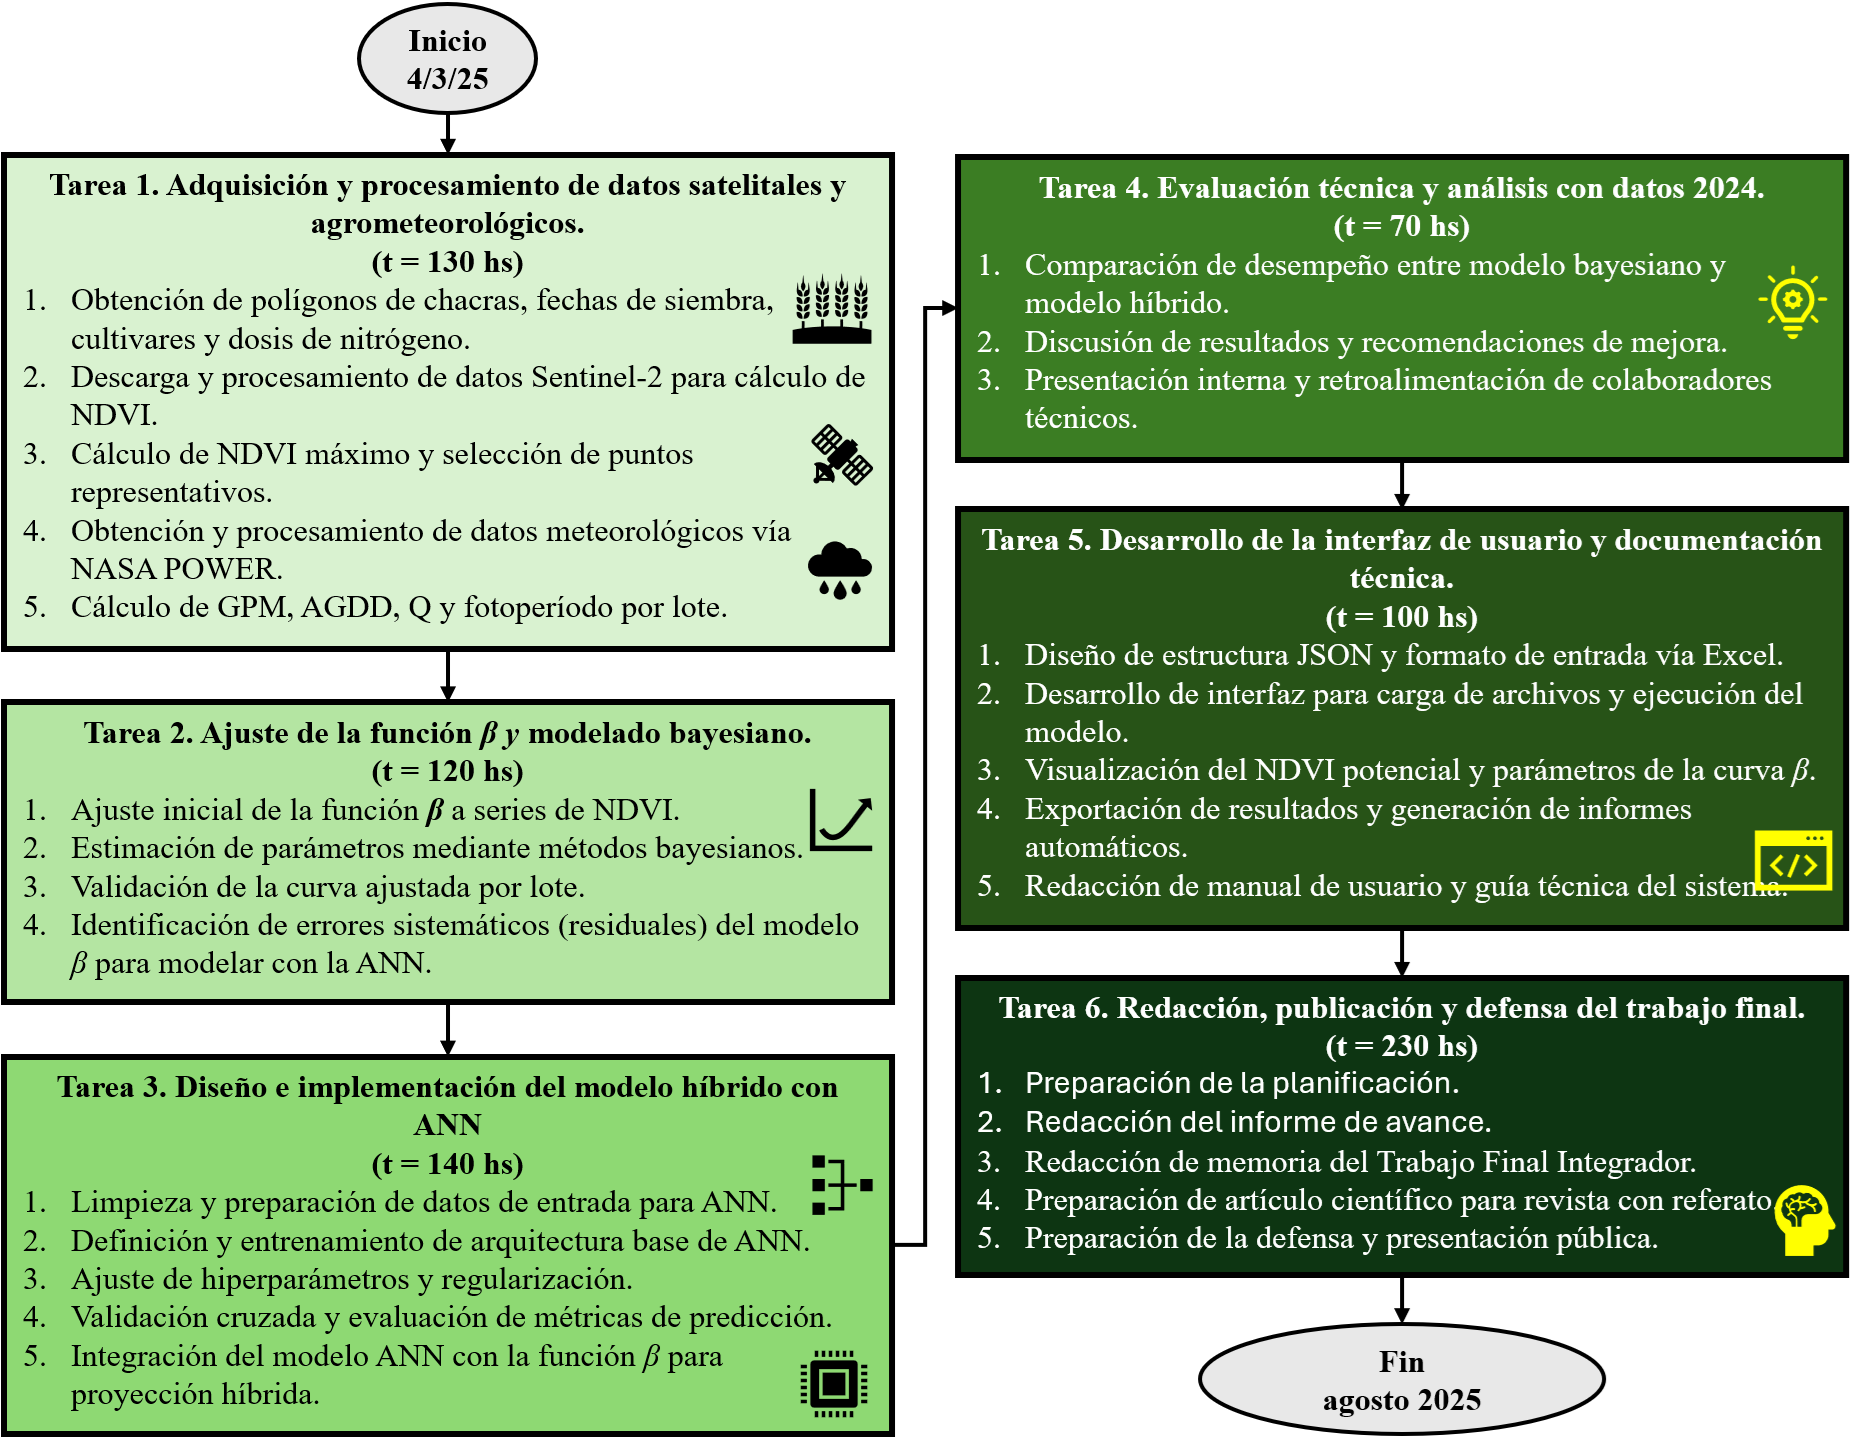
\includegraphics[width=.99
\textwidth]{./Figuras/AoN_ok.png}
\caption{Diagrama de \textit{Activity on Node}.}
\label{fig:AoN}
\end{figure}


El camino crítico, definido como la secuencia de tareas que determina la duración mínima del proyecto, está compuesto por las seis tareas ya descriptas. La duración total estimada del proyecto es de 650 horas, como se resume en el Cuadro~\ref{tab:camino_critico}.

\begin{table}[ht]
\caption{Evolución del camino crítico y acumulación de horas del proyecto}
\label{tab:camino_critico}
\centering
\begin{tabular}{|l|r|}
\hline
\rowcolor[HTML]{C0C0C0}
\textbf{Camino crítico} & \textbf{Horas acumuladas (h)} \\ \hline
T1 $\rightarrow$ T2                                   & 130 \\ \hline
T1 $\rightarrow$ T2 $\rightarrow$ T3                  & 250 \\ \hline
T1 $\rightarrow$ T2 $\rightarrow$ T3 $\rightarrow$ T4 & 370 \\ \hline
T1 $\rightarrow$ T2 $\rightarrow$ T3 $\rightarrow$ T4 $\rightarrow$ T5 & 440 \\ \hline
T1 $\rightarrow$ T2 $\rightarrow$ T3 $\rightarrow$ T4 $\rightarrow$ T5 $\rightarrow$ T6 & 540 \\ \hline
\rowcolor[HTML]{C0C0C0}
TOTAL                                                & 650 \\ \hline
\end{tabular}
\end{table}

\pagebreak


\section{11. Diagrama de Gantt}
\label{sec:gantt}

En la Figura~\ref{fig:Gantt} se presenta el diagrama de Gantt del proyecto, que permite visualizar la planificación temporal de las tareas a lo largo de los seis meses de ejecución comprendidos entre marzo y agosto de 2025. El cronograma se encuentra estructurado en tres grandes bloques que son la organización, ejecución y finalización.

La sección de organización contempla el proceso inicial de planificación del proyecto, el cual se desarrolla en el mes de marzo y abril. A continuación, el bloque de ejecución incluye las seis tareas técnicas principales identificadas en el diagrama de \textit{Activity on Node}, distribuidas secuencialmente desde abril hasta mediados de julio. Esta organización permite respetar las dependencias lógicas entre tareas, minimizar solapamientos y asegurar el cumplimiento del camino crítico identificado previamente.

Finalmente, la etapa de finalización incluye actividades de redacción, revisión y presentación del trabajo final. Se han previsto múltiples versiones del documento (v1, v2 y final), así como instancias clave como el envío de la memoria al director, la elaboración de la presentación y un ensayo general, todo ello alineado con las fechas institucionales estipuladas.

\begin{figure}[htpb]
  \begin{center}
    \begin{ganttchart}[
      time slot unit=day,
      time slot format=isodate,
      x unit=0.06cm,
      y unit title=0.7cm,
      y unit chart=0.6cm,
      milestone/.append style={xscale=4}
      ]{2025-03-01}{2025-08-31}
      \gantttitlecalendar*{2025-03-01}{2025-08-31}{year} \\
      \gantttitlecalendar*{2025-03-01}{2025-08-31}{month} \\
      \ganttgroup{Duración Total}{2025-03-01}{2025-08-31} \\
      %%%%%%%%%%%%%%%%%Organización
      \ganttgroup{Organización}{2025-03-01}{2025-04-15} \\
      \ganttbar{Planificación del proyecto}{2025-03-01}{2025-04-15} \\
      %%%%%%%%%%%%%%%%%Ejecución
      \ganttgroup{Ejecución}{2025-04-16}{2025-07-15} \\
      \ganttbar{Tarea 1}{2025-04-16}{2025-04-30} \\
      \ganttbar{Tarea 2}{2025-05-01}{2025-05-15} \\
      \ganttbar{Tarea 3}{2025-05-16}{2025-05-31} \\
      \ganttbar{Tarea 4}{2025-06-01}{2025-06-15} \\
      \ganttbar{Tarea 5}{2025-06-16}{2025-06-30} \\
      \ganttbar{Tarea 6}{2025-07-01}{2025-07-15} \\
      %%%%%%%%%%%%%%%%%Finalización
      \ganttgroup{Finalización}{2025-07-16}{2025-08-31} \\
      \ganttbar{Memoria v1}{2025-07-16}{2025-07-31} \\
      \ganttbar{Memoria v2}{2025-08-01}{2025-08-15} \\
      \ganttbar{Memoria final}{2025-08-16}{2025-08-25} \\
      \ganttmilestone{Enviar memoria al director}{2025-08-25} \\
      \ganttbar{Elaborar la presentación}{2025-08-26}{2025-08-30} \\
      \ganttmilestone{Ensayo de la presentación}{2025-08-31} \\
    \end{ganttchart}
  \end{center}
  \caption{Diagrama de Gantt del proyecto (marzo–agosto 2025).}
  \label{fig:Gantt}
\end{figure}


\section{12. Presupuesto detallado del proyecto}
\label{sec:presupuesto}
En esta sección se presenta un análisis exhaustivo de los costos asociados al proyecto, desglosados por rubro y expresados en pesos uruguayos (UYU). Los costos directos comprenden aquellas partidas imprescindibles para la ejecución del plan de trabajo, incluyendo honorarios del personal técnico, contratación de consultores, viáticos, pasajes, servicios informáticos y un fondo destinado a imprevistos operativos.

El cuadro~\ref{tab:costos_proyecto} resume el total estimado de inversión directa, donde el mayor porcentaje corresponde a recursos humanos especializados, seguido por servicios técnicos asociados al desarrollo y validación de las herramientas digitales. Este desglose permite identificar los componentes clave del presupuesto y asegurar su trazabilidad durante el ciclo del proyecto. Consultado el 21 de abril del 2025 en la web de INIA: 
\url{https://inia.uy/proyectos/artx20221174588-inia-abinbev-manejo-de-cultivos-y-analisis-de-datos}.

\begin{table}[htbp]
\centering
\caption{Detalle de costos del proyecto en pesos uruguayos (UYU).}
\label{tab:costos_proyecto}
\begin{tabularx}{\linewidth}{|X|c|r|r|}
\hline
\rowcolor[HTML]{C0C0C0}
\multicolumn{4}{|c|}{\textbf{COSTOS DIRECTOS}} \\
\hline
\rowcolor[HTML]{C0C0C0}
Descripción & Cantidad & Valor unitario & Valor total (UYU) \\
\hline
Horas de ingeniería        & 2.880 h &   636 UYU/h & 1.831.634 \\
Consultores                &   125 h  & 1.000 UYU/h &   125.000 \\
Viáticos y estadías        &    20 d  & 2.460 UYU/d  &    49.200 \\
Pasajes                    &    25 u  & 4.920 UYU/u  &   123.000 \\
Servicios     &   100 d  & 1 800 UYU/d  &   180\,000 \\
\hline
\multicolumn{3}{|r|}{\textbf{Subtotal directos}} & 2.308.834 \\
\hline
\rowcolor[HTML]{C0C0C0}
\multicolumn{4}{|c|}{\textbf{COSTOS INDIRECTOS}} \\
\hline
\rowcolor[HTML]{C0C0C0}
Descripción & Cantidad & Valor unitario & Valor total (UYU) \\
\hline
Imprevistos                 & —       & —           &    54.532 \\
\hline
\multicolumn{3}{|r|}{\textbf{Subtotal indirectos}} &    54.532 \\
\hline
\rowcolor[HTML]{C0C0C0}
\multicolumn{3}{|r|}{\textbf{TOTAL GENERAL}} & 2.363.366 \\
\hline
\end{tabularx}
\end{table}


Al tipo de cambio 1 USD son 41,91 UYU (cotización del 21 de abril de 2025, Banco Central del Uruguay: \url{https://www.bcu.gub.uy}). Por lo tanto, el subtotal de costos directos de UYU 2.308.834 equivale a aproximadamente USD 55.090,29,  
y el total general de UYU 2.363.366 a aproximadamente USD 56.391,46.




\section{13. Gestión de riesgos}
\label{sec:riesgos}

La gestión de riesgos es fundamental para asegurar el cumplimiento de los objetivos del proyecto en tiempo, calidad y presupuesto. En esta sección se identifican los principales riesgos que podrían afectar negativamente el desarrollo del trabajo, junto con su evaluación inicial, su priorización según el número de prioridad de riesgo (RPN) y las estrategias de mitigación correspondientes.

\subsection*{a) Identificación de riesgos y estimación de sus consecuencias}

\textbf{Riesgo 1: falta de disponibilidad de imágenes satelitales libres de nubes.}
\begin{itemize}
    \item Severidad (S): 9. El NDVI no puede calcularse con precisión si las imágenes están cubiertas por nubes.
    \item Ocurrencia (O): 7. En la región y fechas críticas es común tener escenas nubladas durante varios días consecutivos.
\end{itemize}

\textbf{Riesgo 2: sobreajuste del modelo de red neuronal artificial (\textit{overfitting}).}
\begin{itemize}
    \item Severidad (S): 8. Disminuye la capacidad predictiva en nuevos datos (campaña 2024).
    \item Ocurrencia (O): 6. Es probable debido al alto número de predictores y la variabilidad interanual.
\end{itemize}

\textbf{Riesgo 3: fallas técnicas en el acceso a las APIs de NASA POWER o Earth Engine.}
\begin{itemize}
    \item Severidad (S): 6. Retrasa el acceso a los datos climáticos y satelitales.
    \item Ocurrencia (O): 5. Son plataformas estables pero ocasionalmente tienen interrupciones o cambios en los endpoints.
\end{itemize}

\textbf{Riesgo 4: limitaciones computacionales en el entrenamiento de modelos.}
\begin{itemize}
    \item Severidad (S): 5. Puede impedir entrenar modelos más complejos como LSTM.
    \item Ocurrencia (O): 4. Depende del acceso a recursos de cómputo de alto rendimiento.
\end{itemize}

\textbf{Riesgo 5: retrasos en la redacción de entregables.}
\begin{itemize}
    \item Severidad (S): 7. Afecta directamente los plazos institucionales.
    \item Ocurrencia (O): 6. Existe alta probabilidad debido a la carga de trabajo y coordinación con colaboradores.
\end{itemize}

\subsection*{b) Tabla de gestión de riesgos: (El RPN se calcula como RPN=SxO)}

\begin{table}[htpb]
\caption{Evaluación de riesgos y número de prioridad de riesgo (RPN).}
\label{tab:riesgos}
\centering
\begin{tabularx}{\linewidth}{@{}|X|c|c|c|c|c|c|@{}}
\hline
\rowcolor[HTML]{C0C0C0} 
\textbf{Riesgo} & \textbf{S} & \textbf{O} & \textbf{RPN} & \textbf{S*} & \textbf{O*} & \textbf{RPN*} \\ \hline
Falta de imágenes sin nubes           & 9 & 7 & 63 & 5 & 4 & 20 \\ \hline
Sobreajuste en modelo ANN             & 8 & 6 & 48 & 5 & 3 & 15 \\ \hline
Fallas técnicas en acceso a APIs      & 6 & 5 & 30 & – & – & –  \\ \hline
Limitaciones computacionales          & 5 & 4 & 20 & – & – & –  \\ \hline
Retrasos en redacción de entregables  & 7 & 6 & 42 & 4 & 3 & 12 \\ \hline
\end{tabularx}
\end{table}


Criterio adoptado: 

Se tomarán medidas de mitigación en los riesgos cuyos números de RPN sean mayores a 30. 

Nota: los valores marcados con (*) en la tabla corresponden luego de haber aplicado la mitigación.


\subsection*{c) Plan de mitigación}

\textbf{Riesgo 1: falta de imágenes sin nubes.}
\begin{itemize}
    \item \textbf{Mitigación:} utilizar interpolación temporal de NDVI mediante la función $\beta$ o datos de otros satélites como Landsat 8 y 9. 
    \item \textbf{S* = 5:} la interpolación reduce significativamente el impacto del NDVI ausente.
    \item \textbf{O* = 4:} menor probabilidad de pérdida total al usar estrategias de suavizado y otros sensores que miden NDVI.
\end{itemize}

\textbf{Riesgo 2: sobreajuste en modelo ANN.}
\begin{itemize}
    \item \textbf{Mitigación:} aplicar regularización (L2 y dropout), validación cruzada estratificada y ajuste automático de hiperparámetros.
    \item \textbf{S* = 5:} la corrección en errores se mantiene pero sin degradar la generalización.
    \item \textbf{O* = 3:} la validación cruzada minimiza la probabilidad de \textit{overfitting}.
\end{itemize}

\textbf{Riesgo 5: retrasos en la redacción de entregables.}
\begin{itemize}
    \item \textbf{Mitigación:} establecer fechas internas de revisión, utilizar herramientas de control de versiones y plantillas estructuradas en \LaTeX.
    \item \textbf{S* = 4:} se reduce el impacto de la demora al tener entregables intermedios.
    \item \textbf{O* = 3:} mayor control sobre tiempos de entrega al distribuir las responsabilidades.
\end{itemize}


\section{14. Gestión de la calidad}
\label{sec:calidad}

Con el fin de asegurar la calidad del producto final y el cumplimiento de los objetivos del proyecto, se seleccionaron diez requerimientos críticos definidos en la Sección \ref{sec:requerimientos}. Para cada uno se detallan las actividades de verificación y validación previstas:

\begin{itemize}
    \item Req \#1.1: el modelo de predicción debe estimar el NDVI potencial en lotes de producción comercial de cebada.
    \begin{itemize}
        \item Verificación: ejecutar pruebas unitarias y de integración con datos históricos (campaña 2024) y calcular el error cuadrático medio (RMSE) y el error absoluto medio (MAE) entre los valores de NDVI proyectados y observados.
        \item Validación: presentar al cliente gráficos comparativos de series temporales de NDVI proyectadas frente a las observadas en lotes representativos para obtener su conformidad.
    \end{itemize}

    \item Req \#1.2: la estimación del NDVI potencial debe estar entre 0,4 y 1,0.
    \begin{itemize}
        \item Verificación: implementar pruebas automatizadas para verificar que los valores de salida del modelo se ubiquen dentro del intervalo de 0,4 a 1,0.
        \item Validación: presentar al cliente histogramas de los valores de NDVI generados por el modelo para confirmar su ajuste al rango agronómico definido.
    \end{itemize}

    \item Req \#1.3: el usuario debe estimar el NDVI potencial trazando el polígono del lote y los datos de fecha de siembra, cultivar (variedad vegetal seleccionada por sus características agronómicas deseables) y fertilización nitrogenada.
    \begin{itemize}
        \item Verificación: realizar pruebas de interfaz de usuario y de la interfaz de programación de aplicaciones con polígonos (\textit{shapes}) y parámetros de ejemplo para verificar la correcta ingesta y el procesamiento adecuado de los datos.
        \item Validación: facilitar al cliente la carga de sus propios polígonos y parámetros reales para confirmar que el sistema produce resultados coherentes y válidos.
    \end{itemize}

    \item Req \#1.4: el tiempo de estimación del NDVI en nuevos datos debe ser rápido.
    \begin{itemize}
        \item Verificación: ejecutar una evaluación de rendimiento (\textit{benchmark}) automatizada para cronometrar el tiempo de ejecución del proceso de predicción sobre un conjunto de 10 lotes representativos y asegurar que cada ejecución finalice en menos de 120 s.
        \item Validación: realizar, junto al usuario, una prueba en la herramienta con datos reales aportados por este y confirmar que la visualización del resultado de la predicción ocurra en menos de 2 minutos.
    \end{itemize}

    \item Req \#1.5: el modelo debe captar las variaciones del NDVI asociadas a diferentes niveles de producción de biomasa y micro‑ambientes dentro de cada lote.
    \begin{itemize}
        \item Verificación: inspeccionar visualmente mapas de NDVI máximo en lotes de prueba para confirmar que los cinco puntos seleccionados (mín, máx, cuantiles) recaigan sobre superficie cultivada y representen adecuadamente la variabilidad espacial observada.
        \item Validación: solicitar al cliente su evaluación sobre si la ubicación de los cinco puntos seleccionados y sus respectivos NDVI potenciales ($w_{\text{max}}$) capturan de forma representativa la diversidad de ambientes productivos dentro de lotes conocidos por él.
    \end{itemize}

    \item Req \#1.6: el sistema debe poder estimar el NDVI potencial para la mayoría de los cultivares.
    \begin{itemize}
        \item Verificación: ejecutar análisis del rendimiento del modelo con un conjunto de datos que incluya múltiples cultivares y verificar las métricas de error específicas para cada uno.
        \item Validación: someter a revisión por parte de un experto agrónomo designado por el cliente las predicciones obtenidas para cultivares clave, con el fin de confirmar su plausibilidad agronómica.
    \end{itemize}

    \item Req \#1.7: los datos de NDVI utilizados para la actualización de la proyección bayesiana deben estar libres de cobertura de nubes y artefactos.
    \begin{itemize}
        \item Verificación: evaluar la regla de filtrado temporal ($NDVI_{actual} < 0.9 \times NDVI_{anterior}$) con series de prueba sin filtros para cuantificar su precisión en la detección de nubes (tasa de aciertos y errores).
        \item Validación: facilitar al cliente la inspección visual de series temporales de NDVI filtradas para certificar la eliminación de datos artefados por nubes y obtener una dinámica del NDVI del cultivo que sea precisa.
    \end{itemize}

    \item Req \#2.1: se elaborará un informe de avance durante con los primeros resultados obtenidos.
    \begin{itemize}
        \item Verificación: revisar con los orientadores y colaboradore el borrador del informe para asegurar la cobertura completa de los hitos alcanzados, la metodología empleada y los resultados preliminares relevantes.
        \item Validación: remitir el informe de avance a los evaluadores externos para su revisión, comentarios y aprobación formal.
    \end{itemize}

    \item Req \#2.2: los resultados deben ser publicados en revistas de investigación locales e internacionales.
    \begin{itemize}
        \item Verificación: asegurar que los manuscritos preparados para sumisión cumplan rigurosamente con las normas de estilo y formato especificadas por las revistas científicas objetivo (incluyendo estructura, citación, figuras y tablas).
        \item Validación: obtener una respuesta editorial (aceptación, solicitud de revisiones mayores/menores, o rechazo) por parte de los comités editoriales de, al menos, dos revistas científicas seleccionadas como potenciales vehículos de publicación.
    \end{itemize}

    \item Req \#2.3: la tesis debe ser publicada de forma abierta al público general, de modo de compartir los resultados en redes sociales y correo electrónico
    \begin{itemize}
        \item Verificación: verificar la correcta deposición del documento final de la tesis en un repositorio digital de acceso abierto reconocido (ej., repositorio institucional del posgrado de la FIUBA) y comprobar la correcta asignación y funcionalidad de un identificador persistente (ej. autor).
        \item Validación: solicitar a un grupo seleccionado de colegas o expertos externos al equipo de proyecto que accedan, descarguen y evalúen la claridad conceptual, la completitud metodológica y la accesibilidad general del documento de tesis publicado en el repositorio.
    \end{itemize}
\end{itemize}


\section{15. Procesos de cierre}    
\label{sec:cierre}

Al finalizar la ejecución del proyecto, se organizará una reunión formal de cierre que tendrá por objetivo evaluar el cumplimiento del plan de trabajo, registrar lecciones aprendidas y agradecer a las personas e instituciones que contribuyeron al desarrollo de la iniciativa. A continuación, se detallan las pautas para llevar a cabo este proceso de cierre.

\begin{itemize}
    \item \textbf{Evaluación del cumplimiento del plan de proyecto:}\\
    La evaluación será liderada por el responsable del proyecto, \authorname, quien revisará en detalle el cumplimiento de las tareas planificadas según el cronograma y los entregables definidos en el documento inicial. Para ello, se utilizarán herramientas de trazabilidad como hojas de seguimiento, versiones del código fuente, registros de commits en GitHub y comparativas entre el plan de Gantt y las fechas efectivas de avance. Se redactará un informe técnico-resumen que incluirá una matriz de cumplimiento de objetivos y entregables, el cual será compartido con el cliente y los orientadores.

    \item \textbf{Identificación de técnicas útiles, problemas y soluciones aplicadas:}\\
    El análisis retrospectivo sobre el proceso metodológico será coordinado por el responsable del proyecto en conjunto con los colaboradores técnicos. Se elaborará un acta de lecciones aprendidas que identificará:
    \begin{itemize}
        \item Las técnicas de modelado (Bayes, ANN) que resultaron más eficientes.
        \item Las herramientas tecnológicas que facilitaron el procesamiento (Earth Engine, PyMC, PyTorch).
        \item Problemas operativos o técnicos (por ejemplo, demoras por nubes, errores en metadatos satelitales) y las soluciones implementadas.
    \end{itemize}
    Este documento se incorporará como anexo en la memoria técnica y será referenciado en las conclusiones finales del proyecto.

    \item \textbf{Organización del acto de agradecimiento:}\\
    La organización del acto de cierre estará a cargo del responsable del proyecto, con apoyo de los orientadores académicos. El evento consistirá en una presentación abierta del sistema desarrollado y de los resultados obtenidos, con invitación extendida a todos los interesados: cliente, colaboradores de INIA, docentes de la FIUBA, y participantes del proyecto AmBev. El acto incluirá un espacio de reconocimiento y agradecimiento formal a los distintos actores y se llevará a cabo en modalidad presencial o virtual, según disponibilidad institucional.\\
    Los gastos logísticos asociados (ej. sala, proyector, refrigerio) serán cubiertos por el presupuesto operativo de INIA o, en su defecto, por fondos personales del autor.
\end{itemize}

Este proceso de cierre asegurará la revisión objetiva del desempeño del proyecto y permitirá capitalizar el aprendizaje para futuras iniciativas en el área de teledetección aplicada a cultivos.

\pagebreak

\section{Referencias}
\label{sec:cierre}

\begin{enumerate}
    % A
    \item Araújo, Bruno O. N., Cáceres, Cintia, Barreto, Lorena y Farías, Pablo. (2022). Crecimiento y rendimiento fisiológico de plantas de cebada producidas bajo manejo de nitrógeno. \emph{Ingeniería e Investigación}, 42(2), e200.

    % B
    \item Baethgen, Walter E. y Christianson, Charles B. (1995). Nitrogen fertilizer effects on growth and yield of barley. \emph{Field Crops Research}, 43(1), 87–99.

    \item Beck, Pieter S. A., Atzberger, Clement, Høgda, Kjell A., Johansen, Bernt y Skidmore, Andrew K. (2006). Improved monitoring of vegetation dynamics at very high latitudes: A new method using MODIS NDVI. \emph{Remote Sensing of Environment}, 100(3), 321–334.

    \item Bending, Niall A., Atkinson, Peter M. y Jarman, Richard J. (2014). Estimating biomass of barley using crop surface models (CSMs) derived from UAV-based RGB imaging. \emph{International Journal of Remote Sensing}, 35(9), 3446–3469.

    \item Berger, Andrés, Gaso, Diego, Ciganda, Víctor y Otero, Alberto. (2013). Evaluación de la dinámica temporal de índices espectrales y su relación con variables biofísicas en trigo para estimación de rendimiento. \emph{X Simposio Brasileiro de Sensoriamento Remoto}.

    \item Berger, Andrés G., Repetto, Daniel, Mazzilli, Sebastián y Fernández, Gerardo. (2024). OPTIFERT-N: Nueva herramienta para optimizar la fertilización nitrogenada en trigo. \emph{Revista INIA}, 77, 10–19.

    \item Bertholdsson, Nils O. (1999). Characterization of malting barley cultivars with more or less stable grain protein content under varying environmental conditions. \emph{European Journal of Agronomy}, 10(1), 1–8.

    \item Bürkner, Paul-Christian. (2018). Advanced Bayesian multilevel modeling with the R package brms. \emph{The R Journal}, 10(1), 395–411.

    % C
    \item Cammarano, Davide, Paruelo, José M., Reussi Calvo, Natalia I. y Sadras, Víctor O. (2024). Impact of nitrogen and water on barley grain yield and malting quality. \emph{Journal of Soil Science and Plant Nutrition}, 24, 6718–6730.

    \item Campbell, J.B., Wynne, R.H. y Thomas, V.A. (2022). \emph{Introduction to remote sensing} (6.ª ed.). The Guilford Press, New York, USA. \url{https://doi.org/10.1117/3.673407.ch1}

    \item Carpenter, B., Gelman, A., Hoffman, M. D., Lee, D., Goodrich, B., Betancourt, M., Brubaker, M. A., Guo, J., Li, P., \& Riddell, A. (2017). Stan: A probabilistic programming language. \emph{Journal of Statistical Software}, 76(1), 1–32. \url{https://doi.org/10.18637/jss.v076.i01}

    \item Cavalli, S., Penzotti, G., Amoretti, M. y Caselli, S. (2023). A Machine Learning Approach for NDVI Forecasting based on Sentinel-2 Data. En \emph{16th International Conference on Software Technologies}, 473–480.

    \item Clark, D. R. (2003). LDF curve-fitting and stochastic reserving: a maximum likelihood approach. En \emph{CAS Forum} (Vol. 3, No. 4, pp. 41–92).

    % E
    \item ESA. (2025). \emph{Sentinel Online - ESA} [sitio web]. Recuperado de \url{https://sentinel.esa.int/web/sentinel/home} [Consulta: 04 de abril de 2025].

    % F
    \item Farbo, A., Sarvia, F., De Petris, S., Basile, V. y Borgogno-Mondino, E. (2024). Forecasting corn NDVI through AI-based approaches using sentinel 2 image time series. \emph{ISPRS Journal of Photogrammetry and Remote Sensing}, 211, 244–261.

    % G
    \item Guszcza, James. (2008). Hierarchical growth curve models for loss reserving. \emph{Casualty Actuarial Society Forum}, Fall, 103–151.

    % H
    \item Halstead, Morgan, Tavarez, Rosa, Thomas, Charles y Smith, Daniel. (2022). Barley grain protein is influenced by genotype, environment, and nitrogen management. \emph{Crop Science}, 63(1), 115–127.

    \item Hu, Yuntao, Barmeier, Gerhard y Schmidhalter, Urs. (2021). Genetic variation in grain yield and quality traits of spring malting barley. \emph{Agronomy}, 11(6), 1177.

    % L
    \item Lapaz Olveira, A.M., Saínz Rozas, H.R., Castro-Franco, M., Carciochi, W.D., Nieto, L., Balzarini, M., Ciampitti, I. y Reussi Calvo, N.I. (2023). Monitoring Corn Nitrogen Concentration from Radar (C-SAR), Optical, and Sensor Satellite Data Fusion. \emph{Remote Sensing}, 15. \url{https://doi.org/10.3390/rs15030824}

    % M
    \item MacLeod, Aaron. (s.f.). \emph{Understanding Malting Barley Quality}. Center for Craft Food and Beverage, Hartwick College. Recuperado de \url{https://www.canr.msu.edu/uploads/234/78941/Understanding_Malting_Barley_Quality_-_Aaron_MacLeod.pdf} [Consulta: 04 de abril de 2025].

    \item Martín, Osvaldo. (2024). \emph{Bayesian Analysis with Python: A Practical Guide to Probabilistic Programming}. Packt Publishing.

    % P
    \item Paruelo, José M., Piñeiro, Germán, Grau, Ricardo y Alcaraz-Segura, David. (2024). Hybrid modeling for grassland productivity prediction: Combining mechanistic models and machine learning. \emph{Ecological Indicators}, 155, 111372.

    \item Paszke, A., Gross, S., Massa, F., Lerer, A., Bradbury, J., Chanan, G., Killeen, T., Lin, Z., Gimelshein, N., Antiga, L., Desmaison, A., Köpf, A., Yang, E., DeVito, Z., Raison, M., Tejani, A., Chilamkurthy, S., Steiner, B., Fang, L., Bai, J., \& Chintala, S. (2019). PyTorch: An Imperative Style, High-Performance Deep Learning Library. \emph{arXiv preprint} \url{arXiv:1912.01703}.

    \item Pettersson, Carl G. y Eckersten, Henrik. (2007). Prediction of grain protein in spring malting barley. \emph{European Journal of Agronomy}, 27, 205–214.

    % R
    \item Reussi Calvo, Natalia I., Carciochi, Walter D. y Prystupa, Pablo. (2022). Economic optimum nitrogen rate analysis for feed and malting barley. \emph{Crop Science}, 62(4), 1997–2010.

    \item Reussi Calvo, Natalia I., Sadras, Víctor O., Cerrudo, Aníbal, Monzón, Juan P. y Abbate, Pedro E. (2020). Canopy indices: A model to estimate the nitrogen rate for barley and wheat. \emph{Journal of Soil Science and Plant Nutrition}, 20, 535–548.

    \item Reussi Calvo, Natalia I., Sadras, Víctor O., Cerrudo, Aníbal, Monzón, Juan P. y Abbate, Pedro E. (2022). Economic optimum nitrogen rate analysis for feed and malting barley. \emph{Crop Science}, 62(2), 937–952.

    % S
    \item Schneider, M. K., Law, R., \& Illian, J. B. (2006). Quantification of neighbourhood-dependent plant growth by Bayesian hierarchical modelling. \emph{Journal of Ecology}, 310–321.

    % Y
    \item Yoosefzadeh-Najafabadi, Majid, Tulpan, Dan y Eskandari, Mostafa. (2021). Using hybrid artificial intelligence and evolutionary optimization algorithms for estimating soybean yield and fresh biomass using hyperspectral vegetation indices. \emph{Remote Sensing}, 13(13), 2555.

    \item Yin, Xinyou, Goudriaan, Jan, Lantinga, Egbert A., Vos, Jan y Spiertz, Hendrik J. (2003). A flexible sigmoid function of determinate growth. \emph{Annals of Botany}, 91(3), 361–371.

\end{enumerate}

\end{document}